\chapter{Tests} \label{sec:evaluation}

In diesem Kapitel sollen die beschriebenen und prototypisch implementierten Verfahren zur Überlagerung gegenübergestellt werden, um anhand eines direkten Vergleichs eine objektive Aussage über die Qualität der Ergebnisse treffen zu können. Hierzu wird im ersten Teil das Vorgehen zum Testen vorgestellt, welches darauf folgend mit allen Verfahren umgesetzt wird. Hiernach werden die daraus resultierenden Ergebnisse gegenübergestellt.

\section{Statische Testszenen}

Zum Vergleich der Verfahren wurden zwei statische Szenen gewählt, in denen das Project Tango Gerät nicht bewegt wird und dadurch allen Kandidaten den selben sensorischen Inhalt bietet. Diese Wahl wurde getroffen, um eine zuverlässige und reproduzierbare Informationsquelle für das Gerät zu schaffen. Denn die Reproduktion eines bewegten und dynamischen Szenarios ist für alle zu vergleichenden Verfahren nur sehr schwer möglich. \\

Eine Idee für ein dynamisches Testszenario war es, alle sensorischen Informationen der Hardware einmal aufzunehmen und eine reproduzierbare simulierte Umgebung dieser Daten zu schaffen. Technologien wie das Robot Operating System (ROS) würden dies ermöglichen, jedoch übersteigt der Aufwand den zeitlichen Rahmen dieser Arbeit. Auch wenn die Firma Bosch eine exemplarische Implementation\footnote{Tango Output to Rosbag Files - https://goo.gl/hhnciZ} für die Aufnahme aller Daten in ROS demonstriert, sind die implementierten Verfahren zu sehr in den API Zyklen der Project Tango Schnittstelle involviert, um diese in kurzer Zeit auf eine Desktop Umgebung zu portieren.\\

Die erste gewählte Szene, welche in Abbildung \ref{fig:static-scene} links zu sehen ist, beinhaltet einen Hocker, in Form eines einfachen  Würfels, und einen Sitzball. Der Sitzball wurde gewählt, um auch runde Formen zur Tiefenaufnahme zu testen, welche gegebenenfalls für die Verfahren schwerer zu rekonstruieren sind. Das Project Tango Gerät ist etwas höher in einem Stativ plaziert. Das virtuelle Objekt wird, wie in Abbildung \ref{fig:static-scene} rechts, zwischen die beiden realen Objekte plaziert, sodass es von beiden Seiten durch die realen Objekte überdeckt wird. \\

\begin{figure}[h]
  \centering
	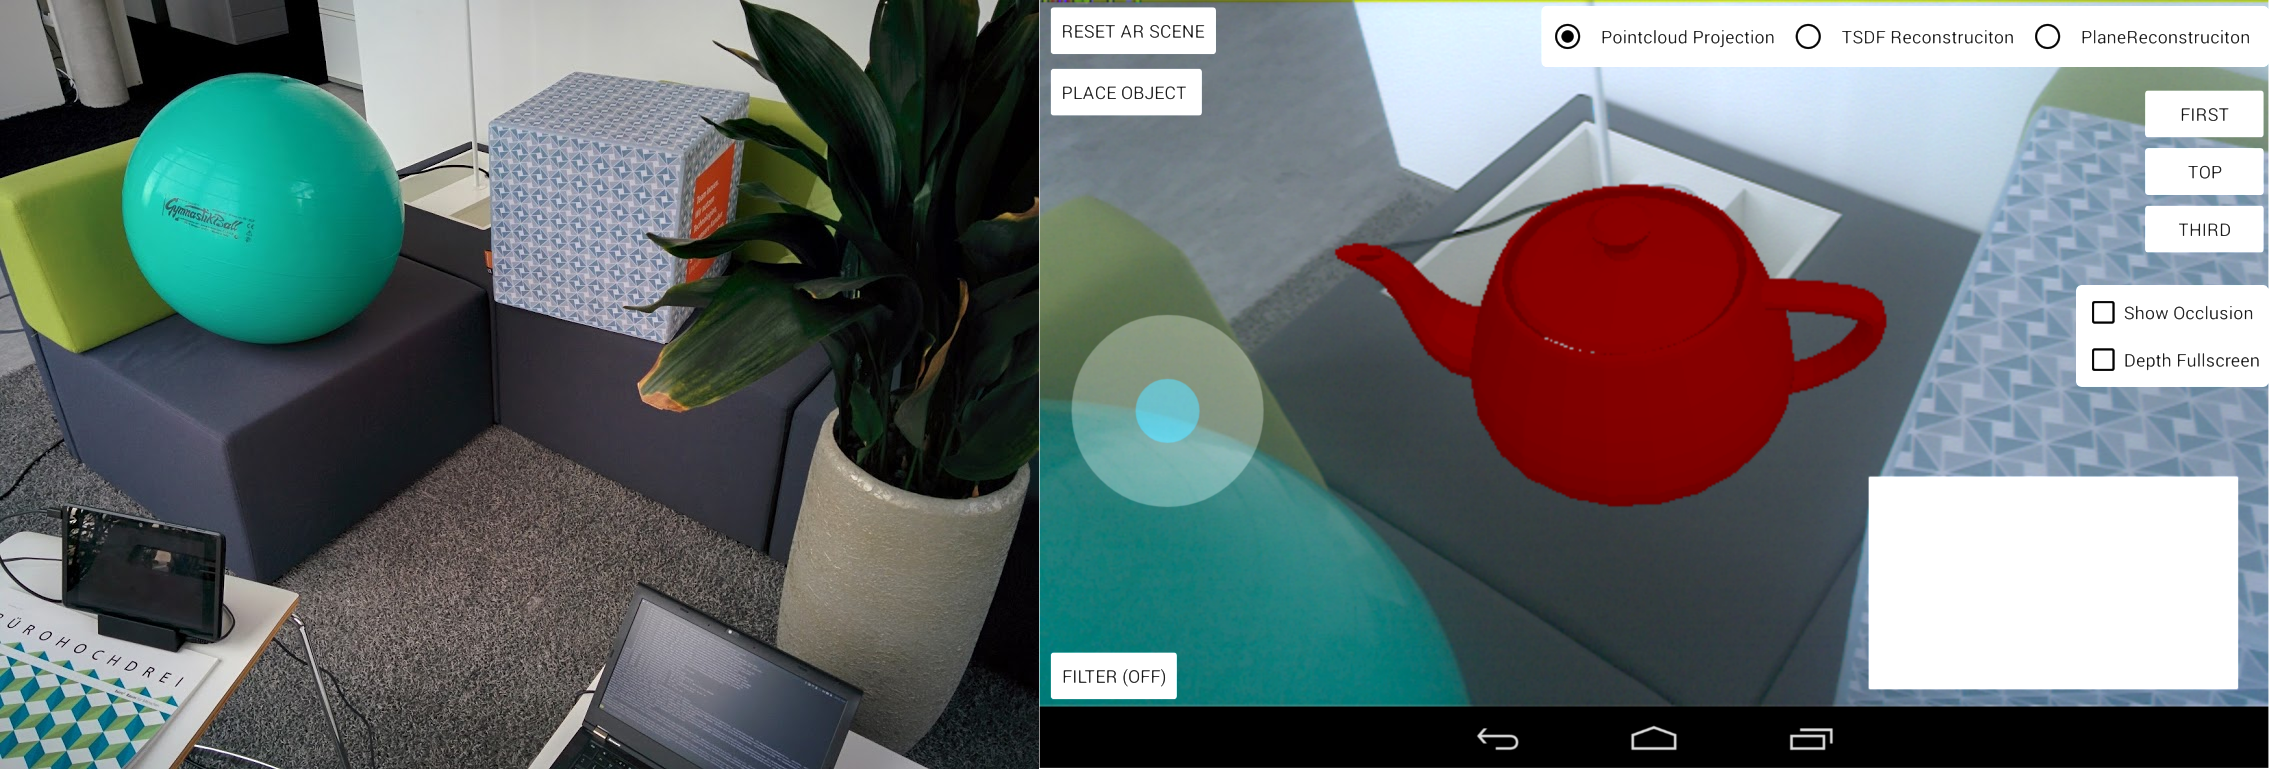
\includegraphics[width=1.0\textwidth]{content/images/evaluation/static-scene.png} 
  \caption{Links: Erste statische Szene mit einem Hocker und einem Sitzball. Rechts: Platzierung des virtuellen Objekts. }
  \label{fig:static-scene}
\end{figure}

Die zweite gewählte Szene, welche in Abbildung \ref{fig:plant-scene} links zu sehen ist, soll als Herausforderung die Überdeckung von komplexeren Strukturen testen. Sie besteht daher aus einer Pflanze, die sich, wie rechts im Bild zu sehen, vor dem virtuellen Objekt befindet. Auch hier befindet sich das Project Tango Gerät in einem Stativ, damit sich die Position während der Tests durch Motion Tracking nicht ändert. \\

\begin{figure}[h]
  \centering
	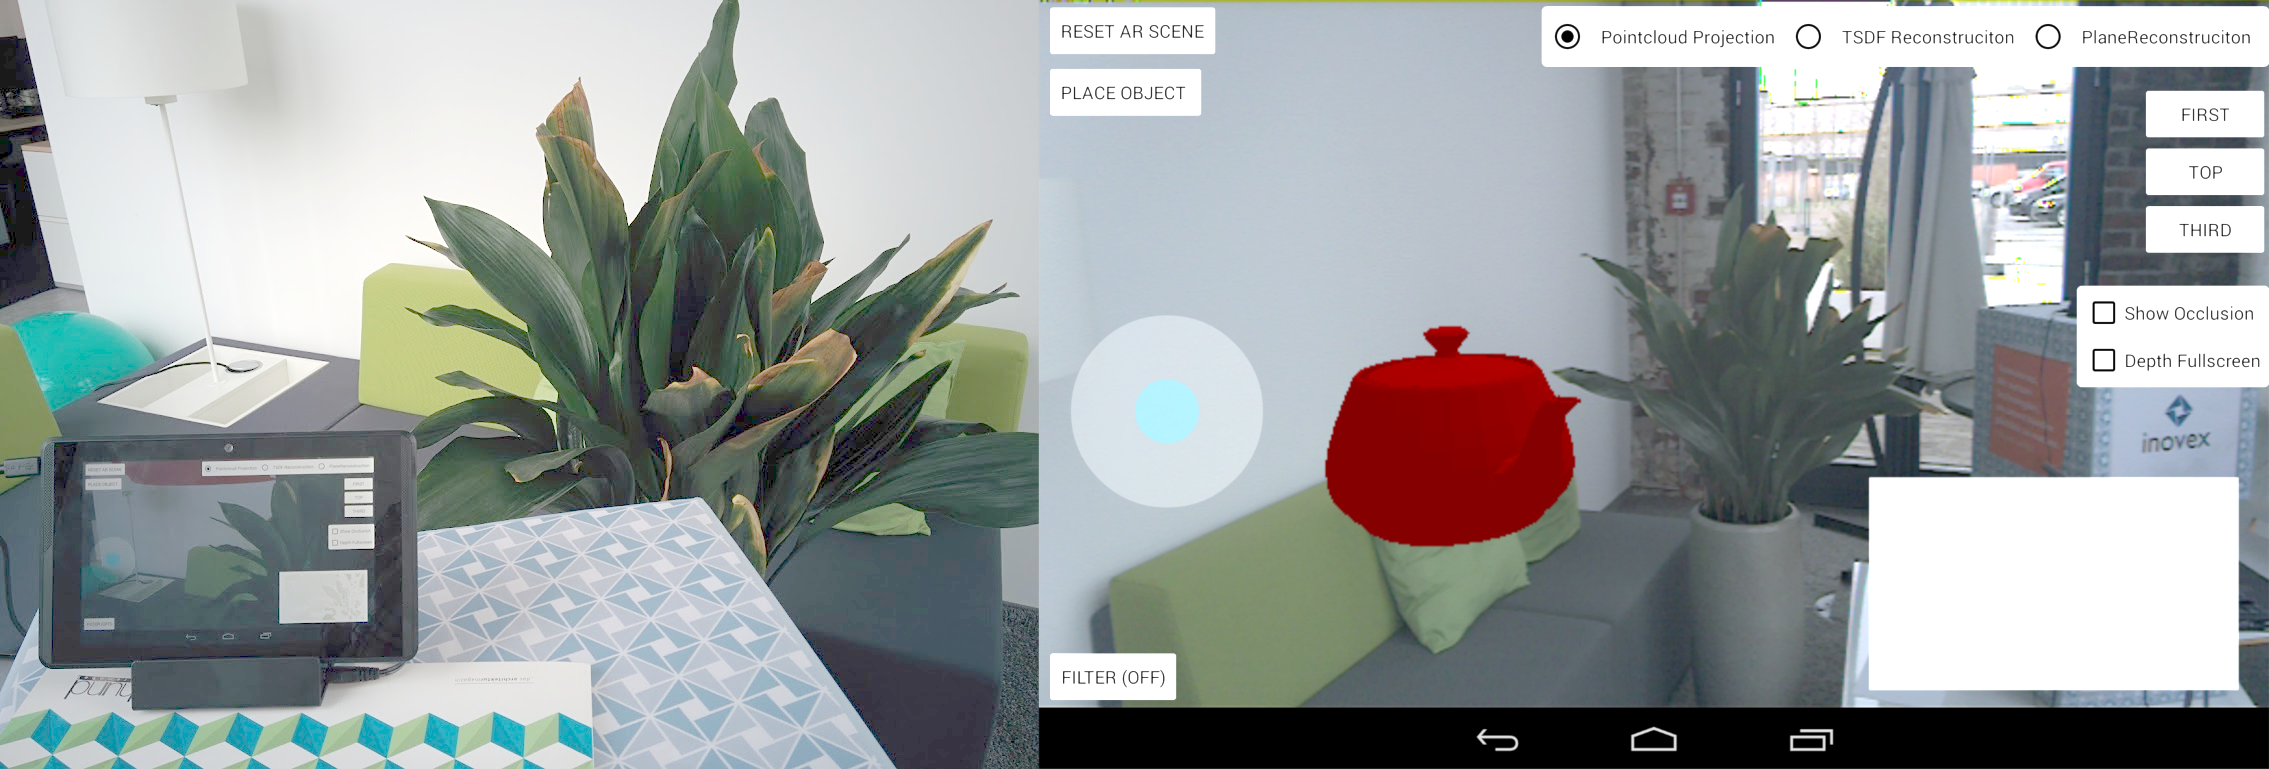
\includegraphics[width=1.0\textwidth]{content/images/evaluation/plant-scene.png} 
  \caption{Links: Zweite statische Szene mit einer Pflanze im Vordergrund. Rechts: Platzierung des virtuellen Objekts hinter der Pflanze. }
  \label{fig:plant-scene}
\end{figure}

Für beide Szenen sollen alle Kombinationen der Verfahren getestet werden. Somit ergeben sich sechs verschiedene Kombinationen, in denen die Pointcloud Projektion, die TSDF Rekonstruktion und die Ebenen Rekonstruktion jeweils mit und ohne der Anwendung des Guided Filter auf das Tiefenbild getestet werden. Für alle Kombinationen soll ein gerendertes Bild und ein Tiefenbild mit dem virtuellen Objekt festgehalten werden. Zur Auswertung werden die jeweils gerenderten Ergebnisbilder \(p\) mit einem manuell zugeschnittenem Ergebnisbild  \(q\) für jeden Pixel \(i\) verglichen. Für diese Gegenüberstellung wird die Summe der absoluten Bilddifferenz wie in Gleichung \ref{eq:diff} bestimmt.

\begin{equation} \label{eq:diff}
d = \sum_i |p_i-q_i|
\end{equation}

\section{Durchführung der Tests}

Die beiden Testszenen konnten wie beschrieben aufgebaut und mit allen Verfahren durchgetestet werden. Hierzu wurde mit der \enquote{Android Debug Bridge} (adb\footnote{Android Debug Bridge - http://goo.gl/ffH51x (01.03.16)}) eine Videoaufnahme gestartet, in der im Prototypen für jede Szene alle Verfahren durchgeschaltet wurden. Die Verfahren mussten dabei sehr schnell gewechselt werden, um einen potentiellen Drift von Project Tangos Motion Tracking so minimal wie möglich zu halten. Denn diese Bewegungen würden die Ergebnisse stark beeinträchtigen. \\

Abbildung \ref{fig:static_occlusion} und \ref{fig:plant_occlusion} im Anhang zeigen jeweils die aus dem Video extrahierten Bildausschnitte. Die obere Reihe zeigt die drei tiefengenerierenden Verfahren ohne den Guided Filter und die untere Reihe jeweils mit dem Filter. In der untersten Reihe sind jeweils die Projektion der generierten Primitiven in der Szene zu sehen, um sich eine Vorstellung der Rekonstruktion machen zu können.

\section{Auswertung der Ergebnisse}

Der Vergleich der Ergebnisse, welcher mit dem bereits beschriebenen Bilddifferenz Ansatz aus der Gleichung \ref{eq:diff} durchgeführt werden soll, wurde mit Hilfe der OpenCV Bibliothek durchgeführt und ist in Listing \ref{lst:compare} zu finden. Für jede Szene wurde ein Referenzbild manuell konstruiert, welches dem idealen Ergebnis entsprechen soll. Diese Referenzbilder sind in Abbildung \ref{fig:reference} zu finden. Mit dem Referenzbild wurden alle zuvor passend zugeschnitten Grafiken einer Szene verglichen. \\

\begin{figure}[h]
  \centering
	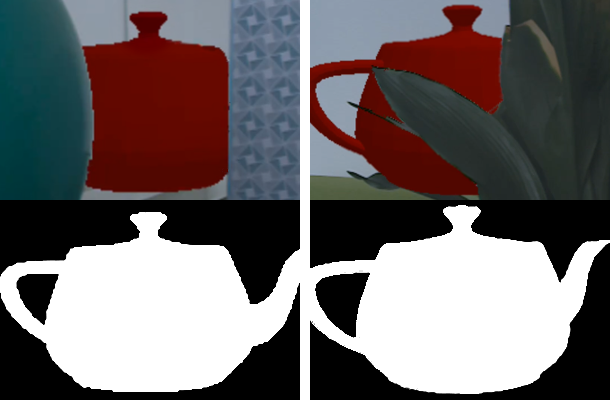
\includegraphics[width=.8\textwidth]{content/images/evaluation/reference.png} 
  \caption{Manuell konstruierte Referenzbilder der idealen Überlagerung in Szene 1 (links) und 2 (rechts).}
  \label{fig:reference}
\end{figure}

Der gezeigte Skript zum Verglich der Ergebnisbilder mit den Referenzbildern ergibt neben den Differenzwerten, welche in Tabelle \ref{tab:results} zu finden sind, auch die absoluten Differenzbilder für jedes Verfahren. Diese Ergebnisbilder sind auch im Anhang in Abbildung \ref{fig:static_occlusion_results} zu finden.\\


\begin{table}[]
\centering
\begin{tabular}{@{}rrrr@{}}
\toprule
                      & \textbf{\begin{tabular}[c]{@{}r@{}}Pointcloud \\ Projektion\end{tabular}} & \textbf{\begin{tabular}[c]{@{}r@{}}TSDF \\ Rekonstruktion\end{tabular}} & \textbf{\begin{tabular}[c]{@{}r@{}}Ebenen \\ Rekonstruktion\end{tabular}} \\ \midrule
\textbf{Szene 1}      & 495.695                                                                    & 560.210                                                                  & 247.327                                                                    \\
\textbf{Szene 1 + GF} & 463.612                                                                    & 79.642                                                                & 166.589                                                                    \\
\textbf{Szene 2}      & 190.473                                                                   & 462.780 & 295.008 \\
\textbf{Szene 2 + GF} & 22.148                                                                 & 339.086 & 264.154 \\ \bottomrule
\end{tabular}
\caption{Distanzwert zwischen dem Referenzbild und den Ergebnisbildern in der jeweiligen Szene}
\label{tab:results}
\end{table}


Neben diesen resultierenden Werten werden im Fazit Kapitel \ref{sec:conclusion} auch anhand einiger dynamischer Tests, mit mehr Bewegung, die implementierten und getesteten Verfahren eingeschätzt. Diese, für die Verfahren nicht reproduzierbaren und deshalb nicht im Detail dokumentierten, Tests beinhalteten eine ähnliche statische Szene, um die sich mit einem Seitenschritt bewegt wurde, um die Genauigkeit der Kantenüberdeckung bei Bewegung gegenüberstellen zu können.